\documentclass[9pt]{beamer}
\usepackage[T1]{fontenc}
\usepackage{lmodern}

\mode<presentation>
\usetheme[footline=empty]{Magicc}

\usepackage{graphicx}
\graphicspath{{figures/}}
\DeclareGraphicsExtensions{.pdf, .png, .jpg}

\usepackage{tikz}

\usepackage{float}
\usepackage{subcaption}
\newenvironment{figure*}%
{\begin{figure}}
{\end{figure}}
\usepackage{amsmath}					%	allows for mathematical symbols
\usepackage{amssymb}					%	defines symbol names for all the math symbols


%\setbeamerfont{caption}{size=\small}
\usepackage[textfont={small}]{caption}
%\captionsetup[sub]{font=small,labelfont={bf,sf}}

% add logo to slide header
\addtobeamertemplate{frametitle}{}{%
\begin{tikzpicture}[remember picture,overlay]
\node[anchor=north east,yshift=2pt] at (current page.north east) {\includegraphics[height=0.75cm]{logo_white}};
\end{tikzpicture}}

% create outline slide at each \section{} (optional)
\AtBeginSection[]{\frame{\frametitle{Outline}\tableofcontents[currentsection]}}

% presentation info
\title[Short Title]{Nonlinear Control Framework for Gimbal and Multirotor in Target Tracking}
\author{Jae Hun Lee}
\institute[MAGICC Lab]{\includegraphics[height=0.5in]{logo_gray}}
\date{\today}

\begin{document}

\begin{frame}
\titlepage
\end{frame}

\begin{frame}{Introduction}
Group objective: To track multiple targets robustly using R-RANSAC.
\linebreak
\linebreak
My objective: To ensure targets are not lost in the camera field of view. Image-based visual servoing (IBVS) provides a good framework.
	\begin{figure}
		\includegraphics[scale=1.5]{ibvs.pdf}
		\caption{Image-based visual servoing block diagram}
	\end{figure}
\end{frame}

\begin{frame}{Introduction}
My question: How can I eliminate the needs for the depth term for visual servoing?
\linebreak
\linebreak
My contributions
\begin{enumerate}
	\item presenting three gimbal control algorithms including newly developed adaptive depth gimbal
	control.
	\item integrating the system for multirotor autonomous target following using R-RANSAC
	tracker and demonstrating the hardware results.
	\item developing the unit vector visual servoing framework for UAV control in target tracking.
\end{enumerate}
\end{frame}

\begin{frame}{Gimbal}
	\begin{figure*}[htbp]
	\centering
	\begin{subfigure}[t]{0.3\textwidth}
		\centering
		\includegraphics[height=1.2in]{phantom3_gimbal.jpg}
		\caption{Ideal}
	\end{subfigure}%
	\begin{subfigure}[t]{0.3\textwidth}
		\centering
		\includegraphics[height=1.2in]{chapter2/gimbal_webcam.jpg}
		\caption{First webcam version}
	\end{subfigure}
	\begin{subfigure}[t]{0.3\textwidth}
		\centering
		\includegraphics[height=1.2in]{chapter2/gimbal.jpg}
		\caption{Custom uEYE camera gimbal}
	\end{subfigure}
	\caption{Gimbals}
	\end{figure*}
\end{frame}

\begin{frame}{Gimbal}
	GImbal algorithms
	\begin{enumerate}
		\item Angle commanding gimbal control (UAV book)
		\item Angular rate commanding gimbal control (Hurak and Rezac)
		
		 - introduces image jacobian for gimbal control
		\item Adaptive depth gimbal control (Me)
		
		 - Model Reference Adaptive Control (MRAC) scheme eliminates the depth term in image jacobian
	\end{enumerate}
\end{frame}

\begin{frame}{Adaptive Depth Gimbal Control}
	\begin{figure*}[htbp]
		\centering
		\begin{subfigure}{0.5\textwidth}
			\centering
			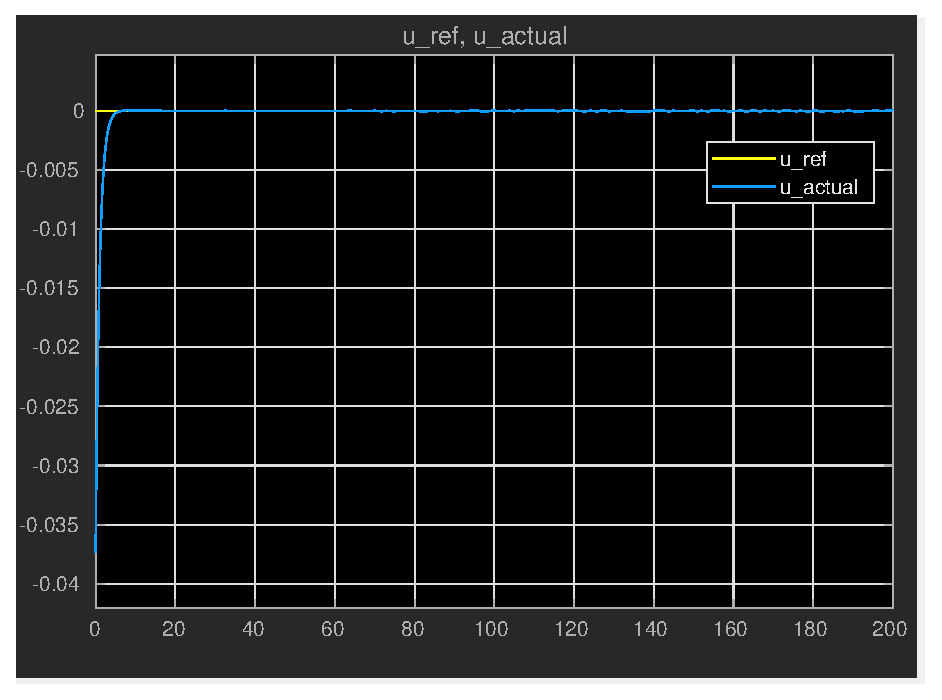
\includegraphics[width=0.8\linewidth]{chapter2/u_adaptive}
			\caption{Reference image coordinate $u_{ref}$ and the system output $u$}
		\end{subfigure}%
		\begin{subfigure}{0.5\textwidth}
			\centering
			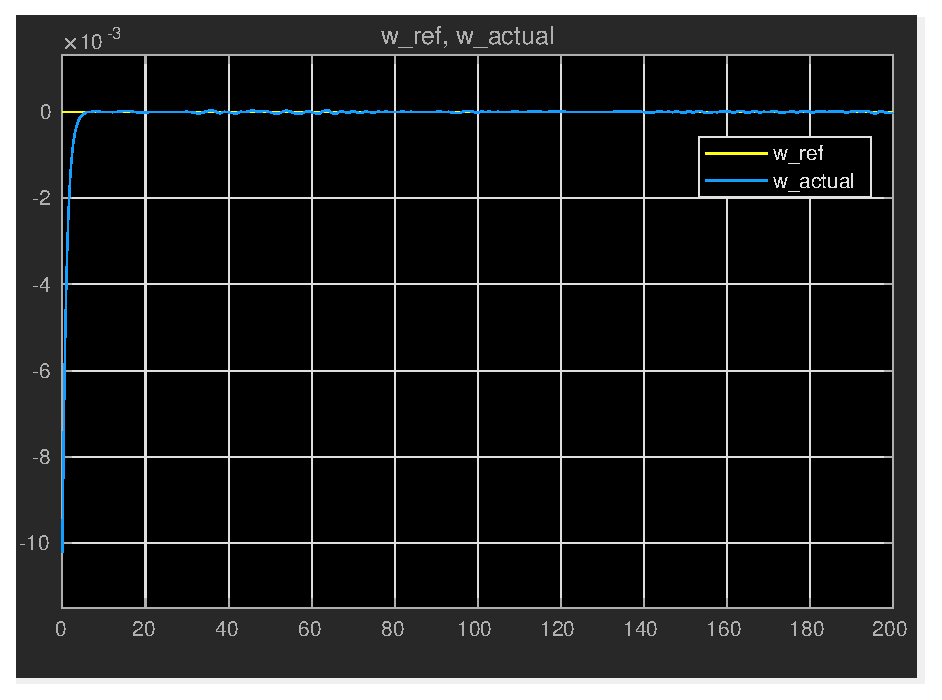
\includegraphics[width=0.8\linewidth]{chapter2/w_adaptive}
			\caption{Reference image coordinate $w_{ref}$ and the system output $w$}
		\end{subfigure}
		\caption{The simulation result for the adaptive depth gimbal control. The system output $u$ and $w$ are converging to the reference model output $u_{ref}$ and $w_{ref}$.}
		\label{adaptive_result}
	\end{figure*}
\end{frame}

\begin{frame}{Adaptive Depth Gimbal Control}
\begin{figure*}[htbp]
	\centering
	\begin{subfigure}{0.5\textwidth}
		\centering
		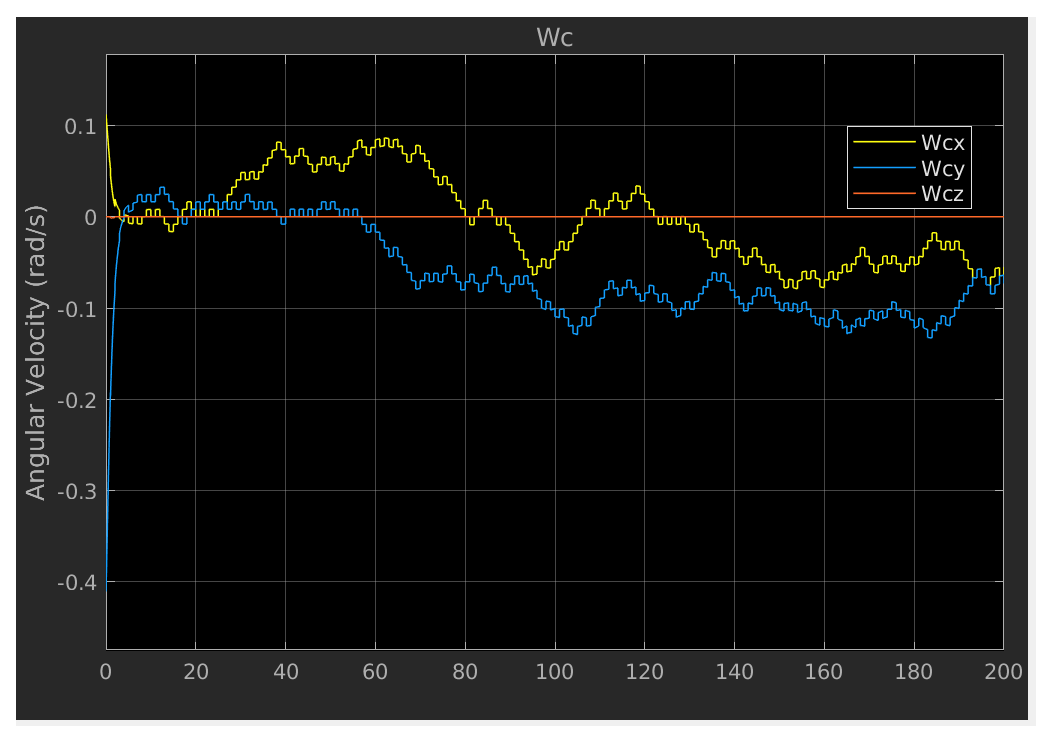
\includegraphics[width=0.8\linewidth]{chapter2/angular_velocity_adaptive}
		\caption{Angular velocity commands}
	\end{subfigure}%
	\begin{subfigure}{0.5\textwidth}
		\centering
		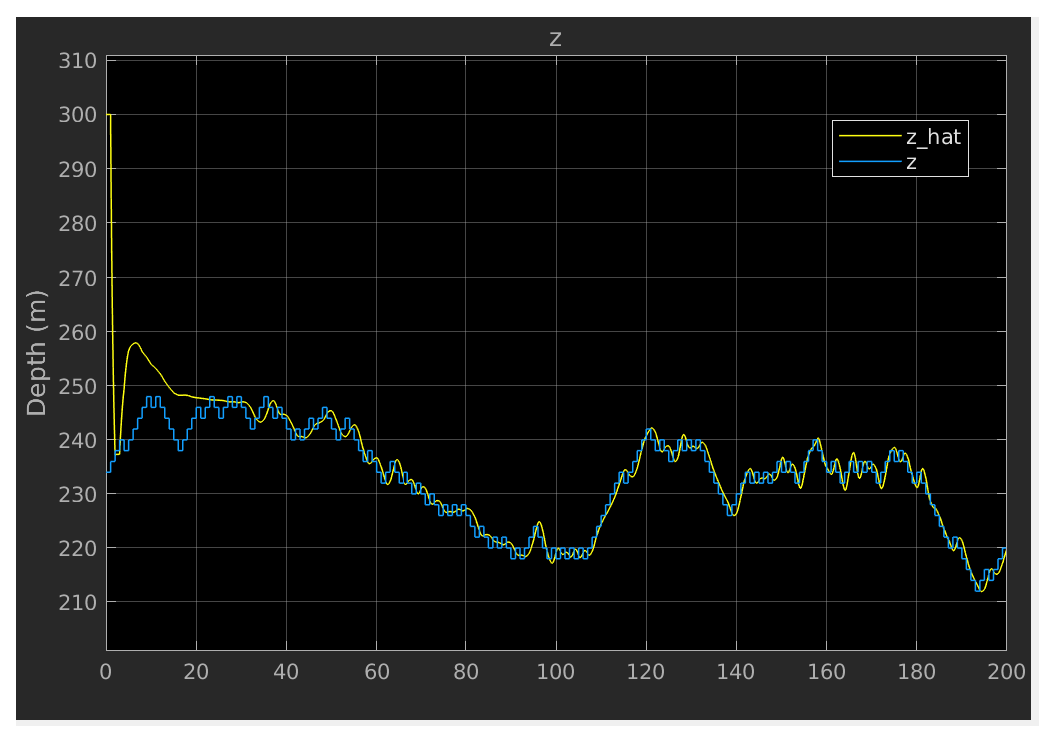
\includegraphics[width=0.8\linewidth]{chapter2/z_adaptive}
		\caption{Online depth estimation, $\hat{z}$}
	\end{subfigure}
	\caption{Angular velocity commands of the adaptive depth gimbal controller. Note that only two commands are used, since it is a pan-tilt gimbal. The depth $z$ estimate using MRAC.}
	\label{adaptive_command}
\end{figure*}	
\end{frame}

\begin{frame}{Adaptive Depth Gimbal Control}
\begin{figure*}[htbp]
	\centering
	\begin{subfigure}{0.5\textwidth}
		\centering
		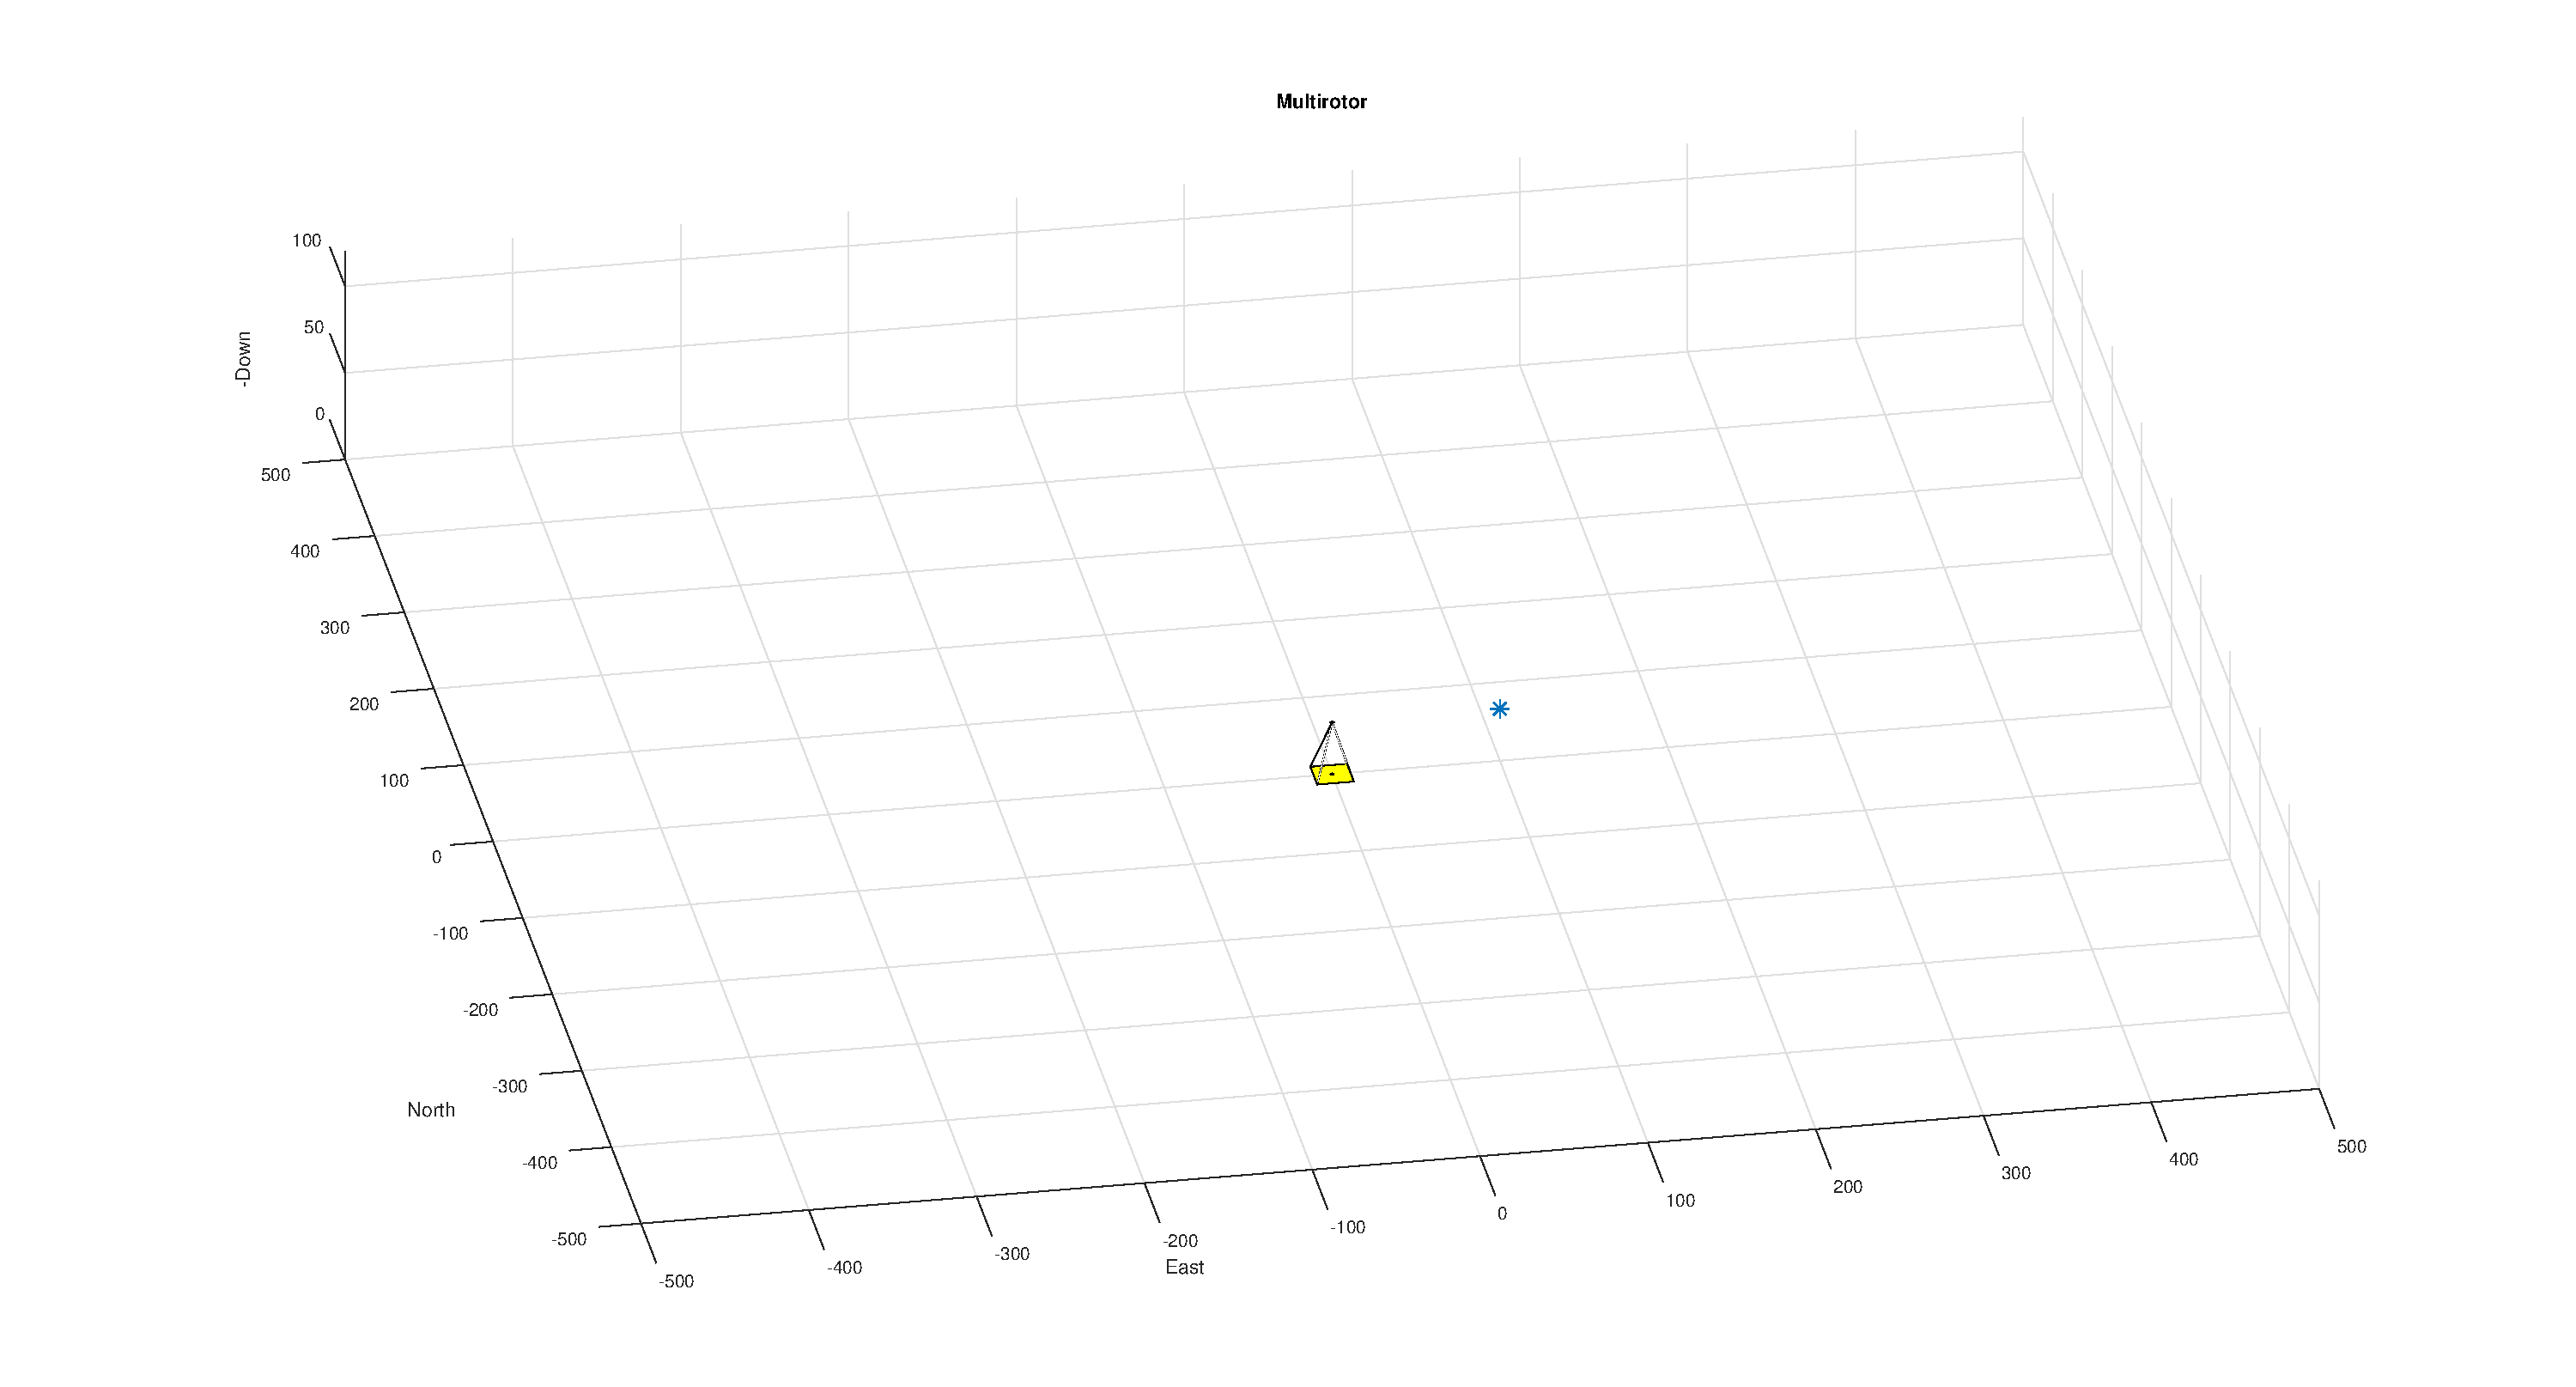
\includegraphics[height=1in]{chapter2/uav_adaptive_0s}
		\caption{Multirotor at $t=0s$.}
	\end{subfigure}%
	\begin{subfigure}{0.5\textwidth}
		\centering
		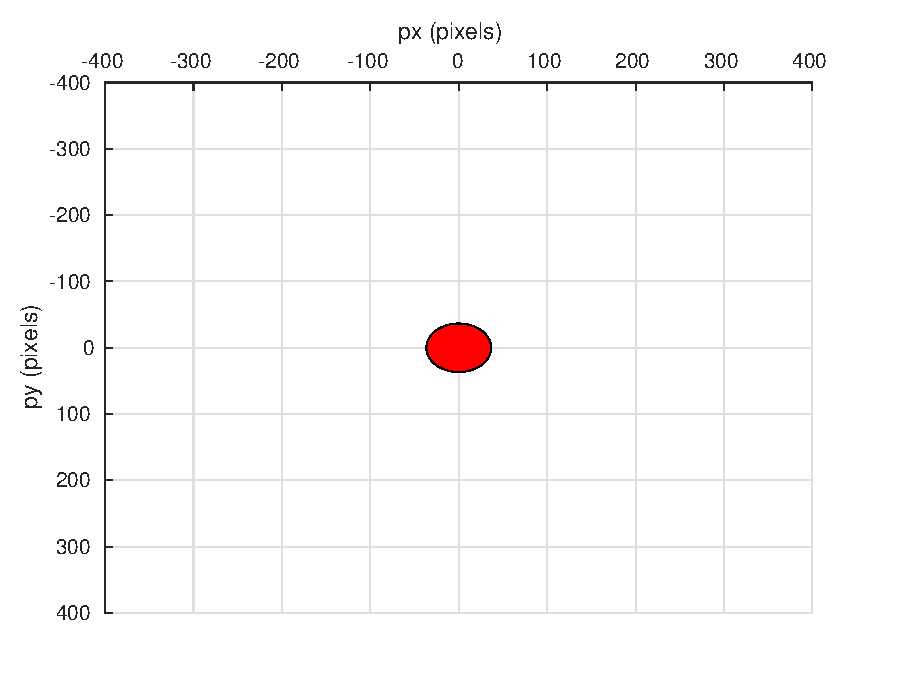
\includegraphics[height=1in]{chapter2/camera_adaptive_0s}
		\caption{Camera view at $t=0s$}
	\end{subfigure}
	\begin{subfigure}{0.5\textwidth}
		\centering
		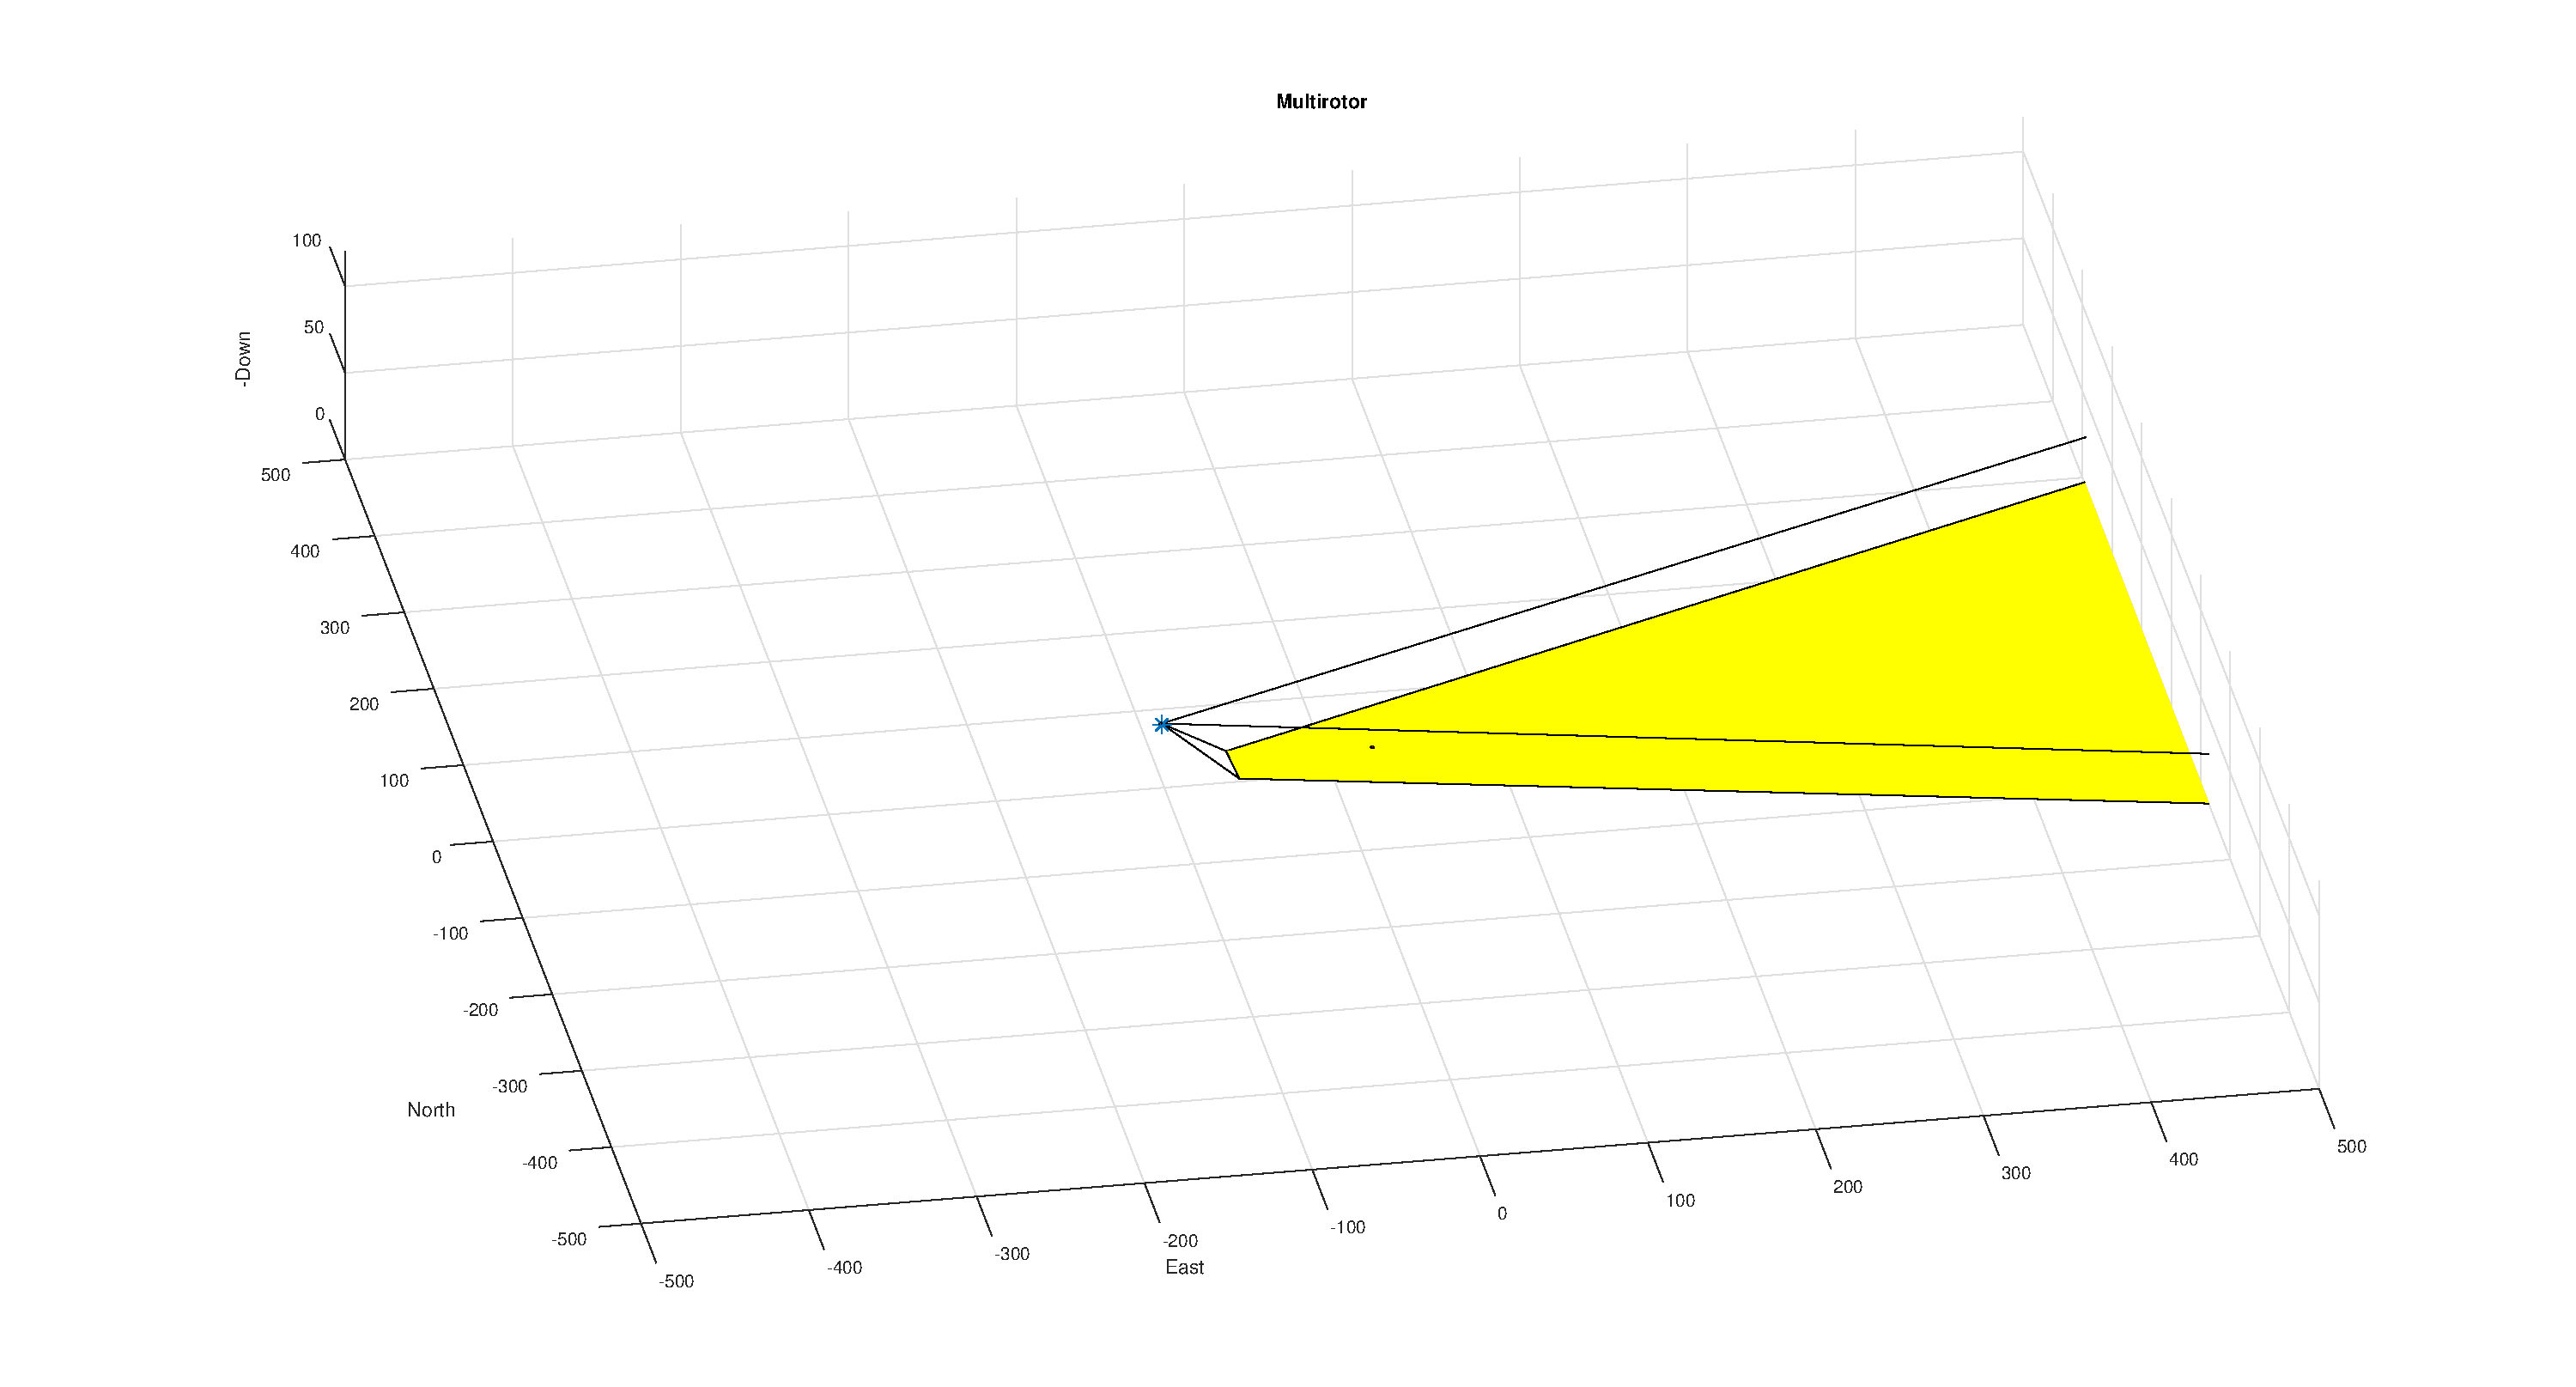
\includegraphics[height=1in]{chapter2/uav_adaptive_180s}
		\caption{Multirotor at $t=180s$}
	\end{subfigure}%
	\begin{subfigure}{0.5\textwidth}
		\centering
		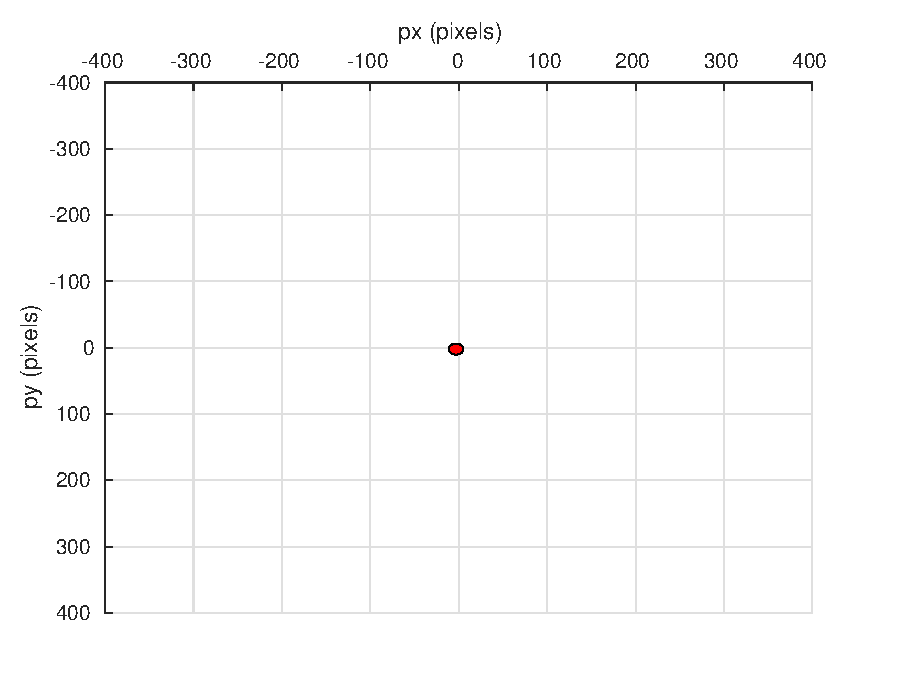
\includegraphics[height=1in]{chapter2/camera_adaptive_180s}
		\caption{Camera view at $t=180s$}
	\end{subfigure}					
	\caption{Multirotor simulation with camera view. The gimbal pointing objective is well achieved.}
	\label{uav_adaptive}
\end{figure*}
\end{frame}

\begin{frame}{Adaptive Depth Gimbal Control}
\begin{figure*}[htbp]
	\centering
	\begin{subfigure}{0.32\textwidth}
		\centering
		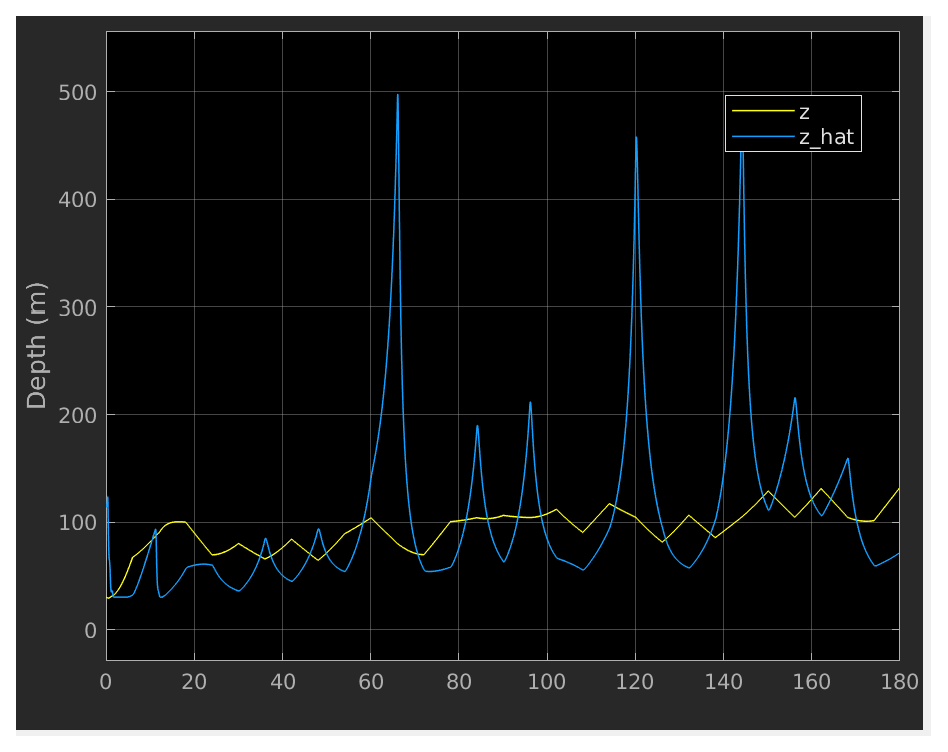
\includegraphics[width=1.4in]{chapter2/uav_z}
		\caption{Depth $z$ and its estimate $\hat{z}$. Uncertain parameter converging to true value is not guaranteed.}
	\end{subfigure}%
	\begin{subfigure}{0.32\textwidth}
		\centering
		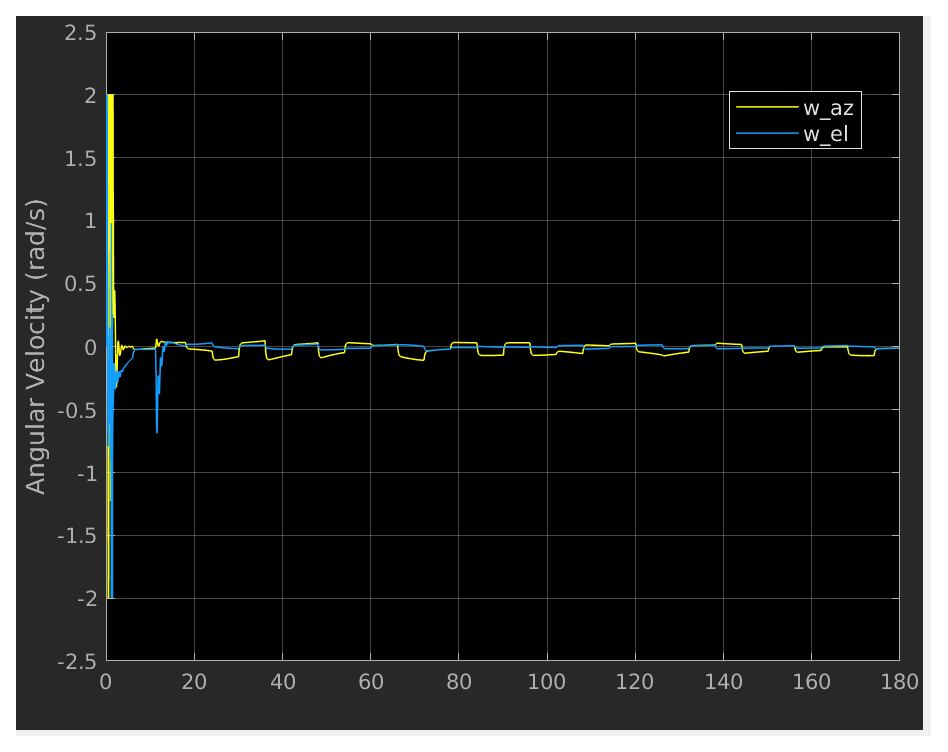
\includegraphics[width=1.4in]{chapter2/uav_gimbal_command}
		\caption{Angular velocity gimbal azimuth and elevation commands}
	\end{subfigure}
	\begin{subfigure}{0.32\textwidth}
		\centering
		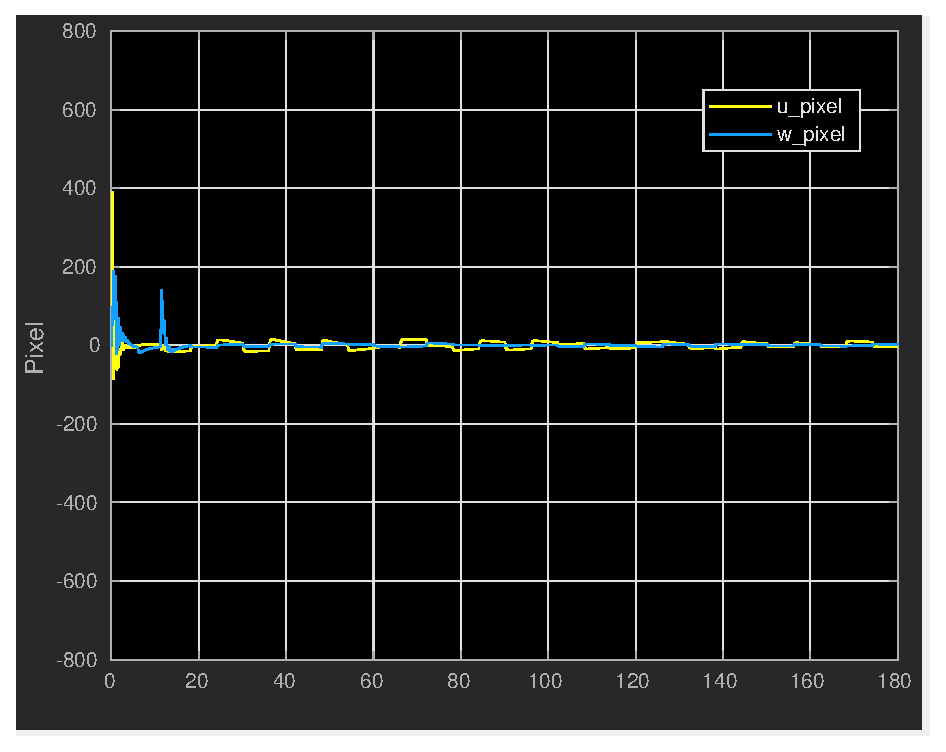
\includegraphics[width=1.4in]{chapter2/uav_pixel}
		\caption{Pixel value $u$ and $w$. They are maintained around the center of the image.}
	\end{subfigure}	
	\caption{Uncertain parameter estimation, gimbal angular velocity commands from the controller, and where target lies in the image.}
	\label{uav_adaptive_additional}
\end{figure*}	
\end{frame}

\begin{frame}{Adaptive Depth Gimbal Control}
\begin{figure}[htbp]
	\centering
	\includegraphics[height=0.8in]{chapter2/gimbal_parts.png}
	\caption{A custom pan-tilt camera gimbal}
	\label{gimbal_parts}
\end{figure}
\begin{figure}[htbp]
	\centering
	\includegraphics[height=0.8in]{chapter2/gimbal_system_blockdiagram}
	\caption{Custom gimbal block diagram}
	\label{gimbal_blockdiagram}
\end{figure}	
\href{https://www.youtube.com/watch?v=VMfvQkhD9-o}{https://www.youtube.com/watch?v=VMfvQkhD9-o}
\end{frame}

\begin{frame}{Gimbal}
ACGC
\begin{itemize}
	\item Easy to implement
	\item Designed for static camera
\end{itemize}
AVCGC
\begin{itemize}
	\item Designed for moving camera
	\item Requires the knowledge of the depth $z$
\end{itemize}
ADGC
\begin{itemize}
	\item Works without knowing $z$
	\item Suitable for small UAV
\end{itemize}
\end{frame}

\begin{frame}{Autonomous Target Following System}
System overview
\begin{figure}[htbp]
	\centering
	\framebox{\includegraphics[height=1.8in]{chapter3/system_diagram.pdf}}
	\caption{System Architecture. The R-RANSAC tracker produces a set of target ID numbers and corresponding pixel locations. The visual-servoing controller outputs the desired position, heading, and yaw rate based on the pixel location of the requested target.}
	\label{system}
\end{figure}
\end{frame}

\begin{frame}{Autonomous Target Following System}
Relatively simple controller using camera geometry
\begin{figure}[thpb]
	\centering
	\framebox{\includegraphics[height=1.8in]{side_view_45deg_2.pdf}}
	\caption{Side view of the multirotor.}
	\label{side_view}
\end{figure}
\end{frame}

\begin{frame}{Autonomous Target Following System}
Hardware results - camera view
\begin{figure}[htbp]
	\begin{subfigure}{0.3\linewidth}
		\centering
		\includegraphics[width=0.95\textwidth]{chapter3/ID51_track_begin.png}
		\caption{Track ID 51 initiated by R-RANSAC tracker (t=0s)}
		\label{camera1}
	\end{subfigure}
	\begin{subfigure}{0.3\linewidth}
		\centering
		\includegraphics[width=0.95\textwidth]{chapter3/ID51_follow_begin.png}
		\caption{The human operator has commanded the UAV to follow track ID 51 (t=13s)}
		\label{camera2}
	\end{subfigure}
	\begin{subfigure}{0.3\linewidth}
		\centering
		\includegraphics[width=0.95\textwidth]{chapter3/ID65_track_begin.png}
		\caption{Track ID 65 initiated by R-RANSAC tracker (t=27s)}
		\label{camera3}
	\end{subfigure}
	\begin{subfigure}{0.3\linewidth}
		\centering
		\includegraphics[width=0.95\textwidth]{chapter3/ID65_follow_begin.png}
		\caption{The human operator has commanded the UAV to follow track ID 65 (t=35s)}
		\label{camera4}
	\end{subfigure}
	\centering
	\begin{subfigure}{0.3\linewidth}
		\centering
		\includegraphics[width=\textwidth]{chapter3/ID65_following.png}
		\caption{A snapshot of the track ID 65 being followed (t=60s)}
		\label{camera5}
	\end{subfigure}
	\caption{Camera view at various events}
	\label{camera}
\end{figure}	
\end{frame}

\begin{frame}{Autonomous Target Following System}
Hardware results - target footage in image and multirotor GPS footage
\begin{figure*}[htbp]
	\centering
	\begin{subfigure}{0.32\textwidth}
		\centering
		\includegraphics[width=1.4in]{chapter3/ID65_follow_begin_annotated.png}
		\caption{Tracks movement in the normalized image plane. Each event (1)-(4) corresponds to camera view in \ref{camera1}-\ref{camera4} respectively. Until the command to follow ID 65, the multirotor keeps the track ID 51 from leaving the camera view.}
	\end{subfigure}%
	\begin{subfigure}{0.32\textwidth}
		\centering
		\includegraphics[width=1.4in]{chapter3/ID65_trace_annotated.png}
		\caption{The movement of track ID 65 in the normalized image plane. Each event (3)-(5) corresponds to camera view in \ref{camera3}-\ref{camera5} respectively. The controller keeps the track ID 65 in the camera field of view after receiving the command to do so from the human operator.}
	\end{subfigure}
	\begin{subfigure}{0.32\textwidth}
		\centering
		\includegraphics[width=1.4in]{chapter3/GPS_trace.png}
		\caption{Multirotor GPS footage and heading corresponding to camera view in \ref{camera1}-\ref{camera5} respectively.}
	\end{subfigure}	
\end{figure*}	
\end{frame}

\begin{frame}{Unit Vector UAV Visual Servoing}
Motivation
\begin{figure}[htbp]
	\centering
	\framebox{\includegraphics[height=1.5in]{chapter4/advanced_control_motivation.pdf}}
	\caption{Non-flat-earth model example. The unit optical axis vector $\hat{m}$ and the unit line of sight vector $\hat{\ell}$ are key components of the controller presented in this chapter.}
	\label{nonflatearth}
\end{figure}
\end{frame}

\begin{frame}{Unit Vector UAV Visual Servoing}
Control objective
\begin{figure}[htbp]
	\centering
	\framebox{\includegraphics[width=0.2\textwidth]{chapter4/projection.pdf}}
	\caption{Projection onto the null space of the optical axis unit vector}
	\label{projection}
\end{figure}
$$P_{\hat{m}}=(I-\hat{m}\hat{m}^\top)$$
$$\hat{e}_1=[1 \quad 0 \quad 0]^\top$$
$$e_x=\hat{e}_1^{\top}P_{\hat{m}}\hat{\ell}$$
\end{frame}

\begin{frame}{Unit Vector UAV Visual Servoing}
Simulation results - simple dynamics
\begin{figure}[htbp]
	\centering
	\begin{subfigure}[t]{0.32\linewidth}
		\includegraphics[width=1.5in]{chapter4/simple_zero}
		\caption{when $t=0s$}
	\end{subfigure}
	\begin{subfigure}[t]{0.32\linewidth}
		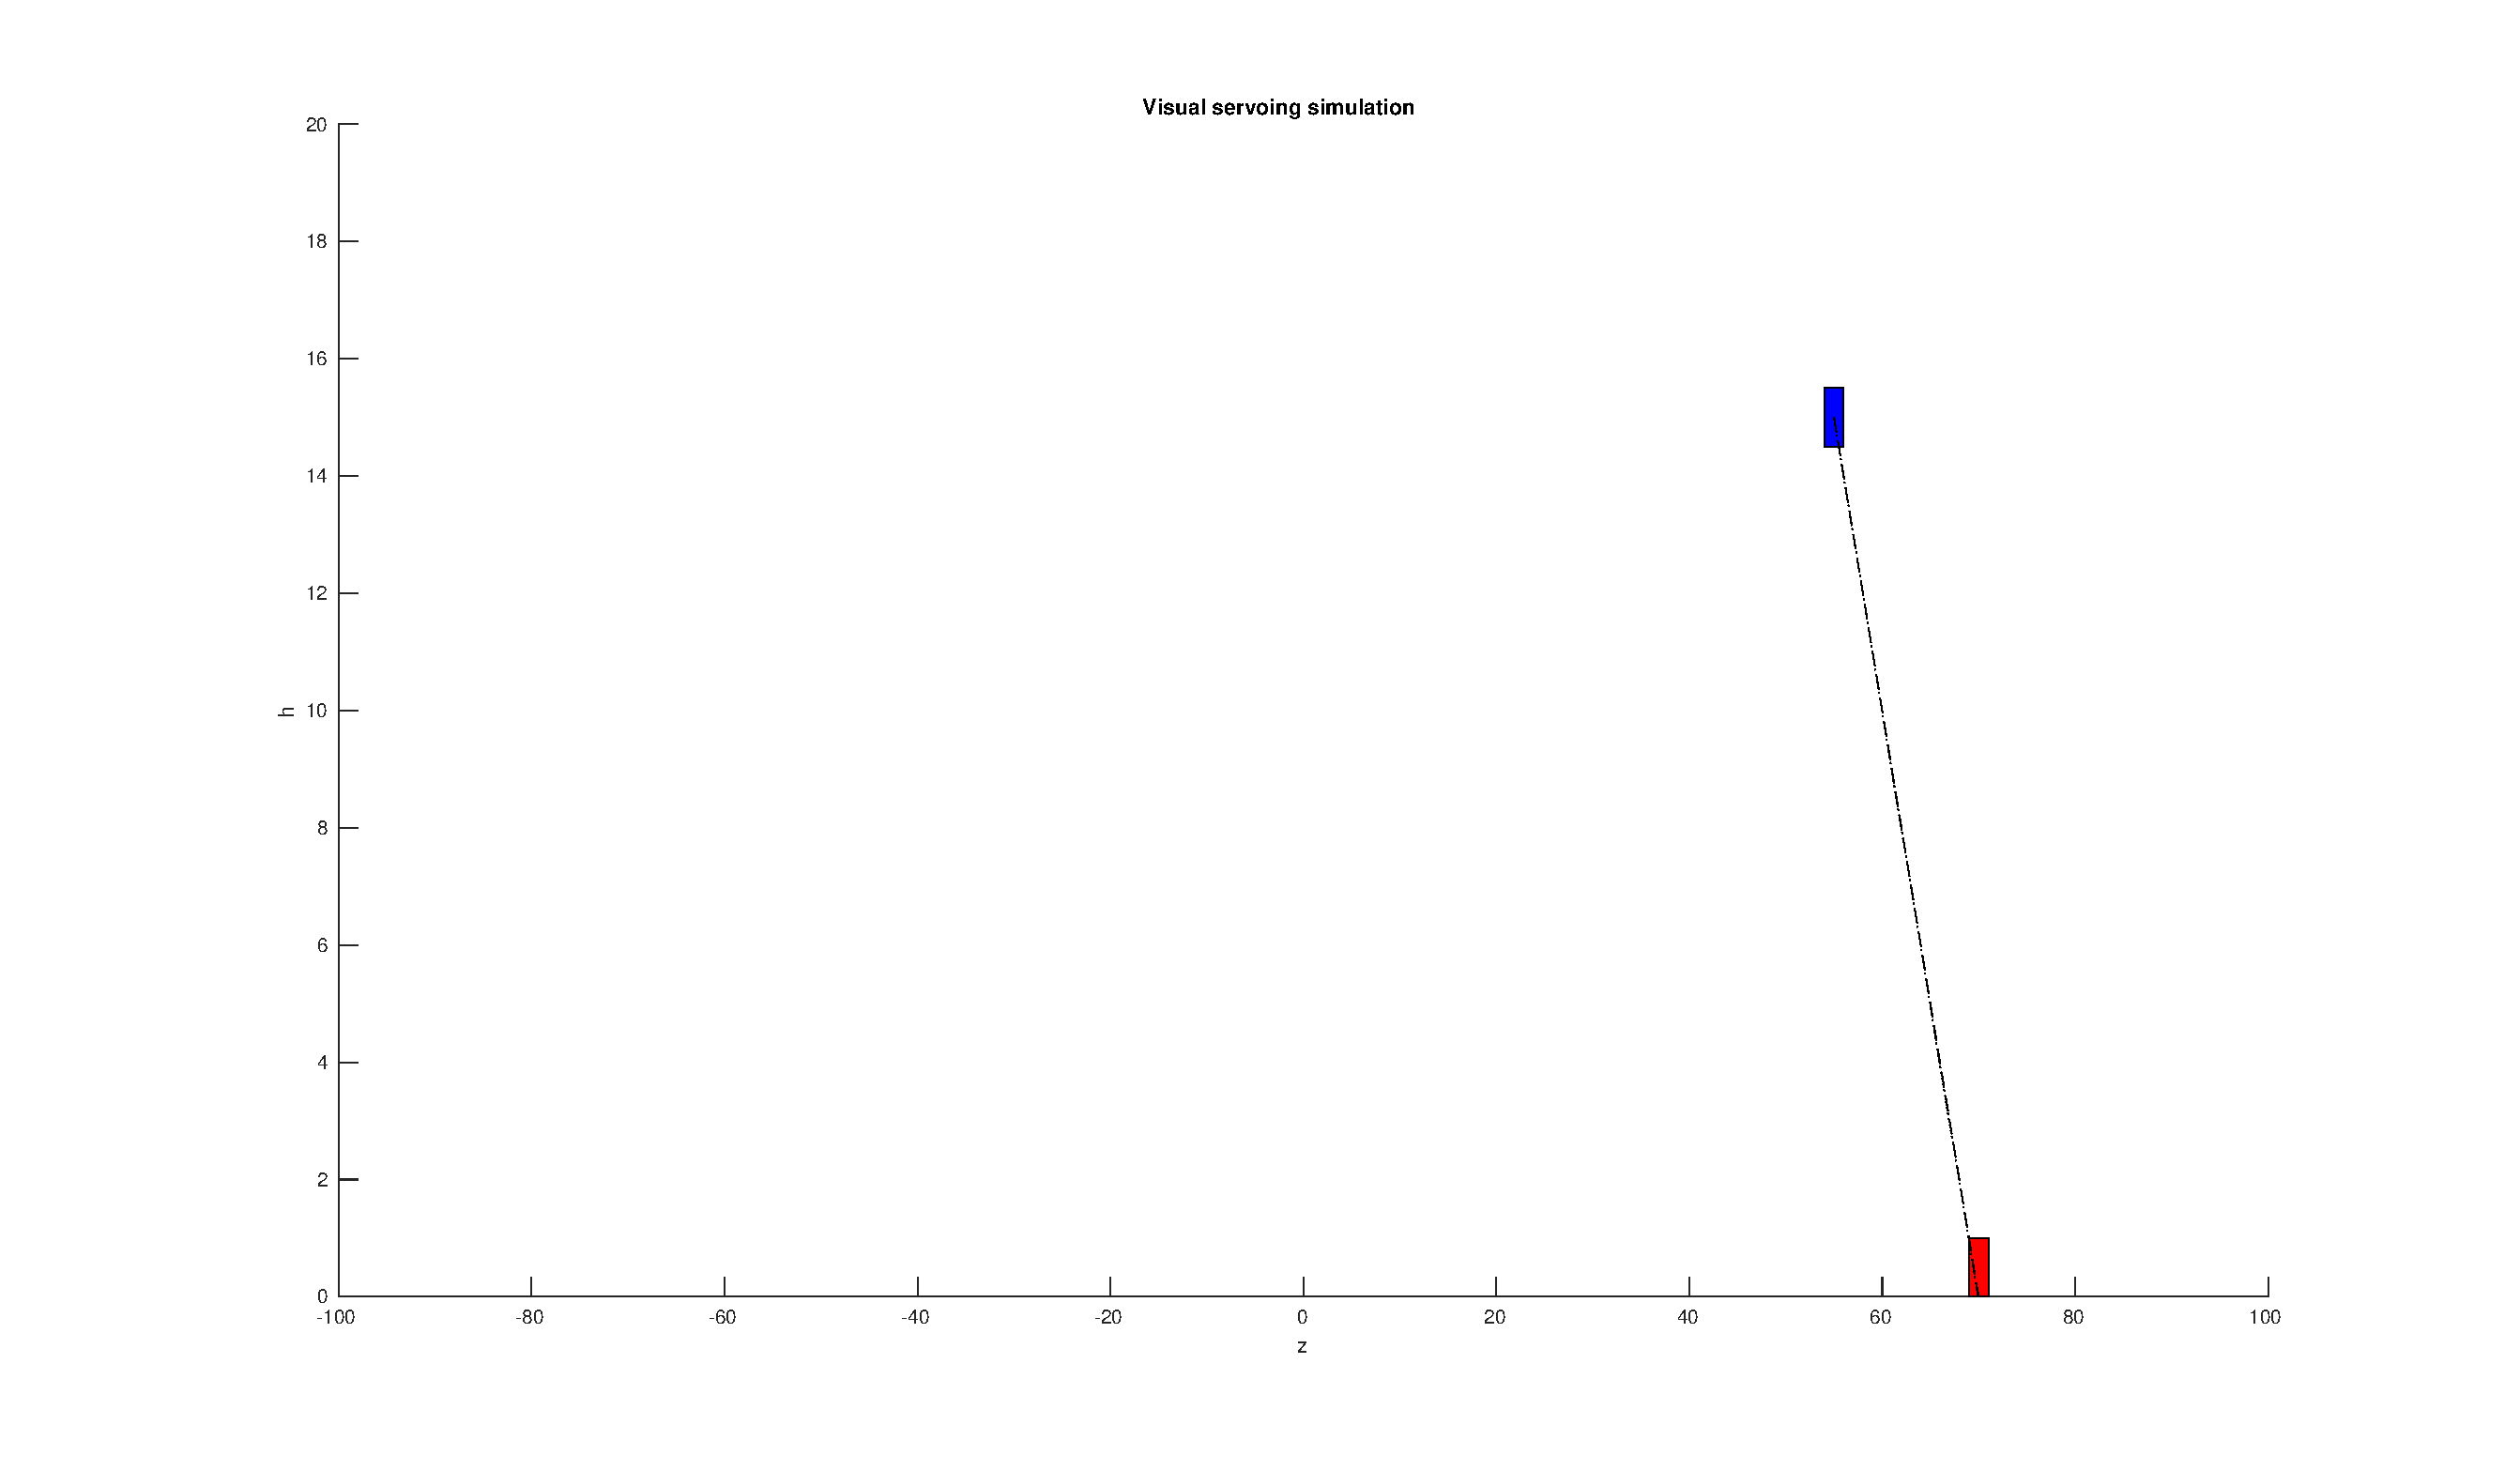
\includegraphics[width=1.5in]{chapter4/simple_ten}
		\caption{when $t=10s$}
	\end{subfigure}
	\begin{subfigure}[t]{0.32\linewidth}
		\centering
		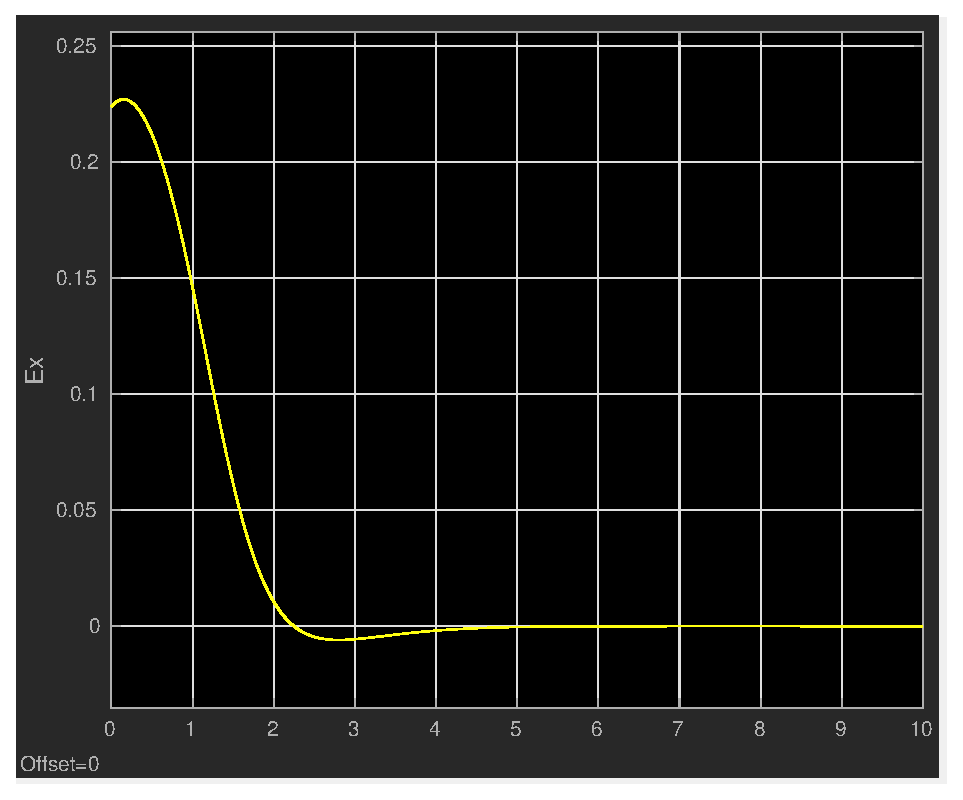
\includegraphics[width=1.5in]{chapter4/simple_ex}
		\caption{The horizontal error between the unit LOS vector and the unit optical axis vector converges to zero.}
	\end{subfigure}	
	\caption{Simple UAV dynamics visual servoing Simulink simulation. The blue square is flying UAV at constant altitude and the red square is a target on the ground moving at $5m/s$. The initial UAV and target positions are [-10, 15] and [20, 0] respectively. Tuning parameters are set to $k=1$, $\Gamma=I_3$ (identity matrix), and $\alpha=1000$.}
	\label{simple_simulation}
\end{figure}
\end{frame}

\end{document}
